\documentclass[oneside,final]{hcmut-report}

\usepackage{array,longtable,tabularx,multirow}
\usepackage{enumitem}
\usepackage{caption,float}
\usepackage[export]{adjustbox}
\usepackage{ragged2e}
\usepackage{tikz}
\usetikzlibrary{arrows.meta,positioning,shapes.geometric}
\usepackage[nameinlink]{cleveref}

\captionsetup{font=small,labelfont=bf}
\setlist[itemize]{itemsep=2pt,topsep=4pt}
\setlist[enumerate]{itemsep=2pt,topsep=4pt}
\newcolumntype{Y}{>{\RaggedRight\arraybackslash}X}
\newcolumntype{L}[1]{>{\RaggedRight\arraybackslash}p{#1}}
\newcommand{\filepath}[1]{\begingroup\footnotesize\ttfamily\path{#1}\endgroup}
\emergencystretch=2em
\sloppy

\AtBeginDocument{
  \renewcommand{\contentsname}{Mục lục}
  \renewcommand{\listfigurename}{Danh sách hình}
  \renewcommand{\listtablename}{Danh sách bảng}
  \renewcommand{\figurename}{Hình}
  \renewcommand{\tablename}{Bảng}
  \renewcommand{\refname}{Tài liệu tham khảo}
}

\deptname{Khoa Khoa học và Kỹ thuật Máy tính}
\coursename{Đồ án Đa ngành hướng Trí tuệ Nhân tạo}
\reporttype{Báo cáo đề tài}
\title{Hệ Thống Cảnh Báo Vật Cản Bằng Giọng Nói Cho Người Khiếm Thị Ứng Dụng Mạng TinyML}
\advisor{& Tiến sĩ Võ Tuấn Bình &}
\stuname{%
  & Nguyễn Đăng Hiên & 2310936 \\
  & Lê Nguyễn Kim Khôi & 2311671 \\
  & Bùi Ngọc Phúc & 2312665 \\
  & Hồ Anh Dũng & 2310543 \\
  & Cao Hữu Thiên Hoàng & 2311030 \\
}
\reportplace{Thành phố Hồ Chí Minh}
\reporttime{Tháng 5 năm 2026}
\makeatletter
\renewcommand{\@upperuniname}{Đại học Quốc gia Thành phố Hồ Chí Minh}
\renewcommand{\@uniname}{Trường Đại học Bách khoa}
\makeatother

\begin{document}
\coverpage

\section*{Tóm tắt}
\addcontentsline{toc}{section}{Tóm tắt}
Đề tài xây dựng hệ thống cảnh báo vật cản bằng giọng nói cho người khiếm thị, sử dụng camera để thu nhận hình ảnh phía trước, mô hình EfficientDet-Lite0 để nhận diện vật thể và Decision Engine để chọn cảnh báo quan trọng nhất. Hệ thống tập trung vào pipeline tích hợp trên thiết bị biên: thu nhận ảnh, suy luận object detection, lọc vật thể liên quan đến an toàn di chuyển, ước lượng mức gần--xa tương đối, xác định hướng trái--giữa--phải và chuyển kết quả thành cảnh báo ngắn gọn.

Trong repository hiện tại, ESP32-CAM đóng vai trò nguồn camera mạng và phát luồng MJPEG qua Wi-Fi; mô hình AI chạy trên Raspberry Pi hoặc máy tính thử nghiệm bằng Python, MediaPipe và Flask. Do đó, thuật ngữ TinyML trong báo cáo được hiểu theo hướng dùng mô hình nhẹ và triển khai suy luận ở biên, không khẳng định mô hình đã chạy trực tiếp trên vi điều khiển ESP32-CAM. Báo cáo trình bày bối cảnh, cơ sở công nghệ, yêu cầu hệ thống, kiến trúc, thuật toán ra quyết định, cấu trúc phần mềm, quy trình demo, kế hoạch kiểm thử và những hạn chế cần cải thiện trước khi đánh giá khả năng sử dụng thực tế.
\clearpage

\tableofcontents
\listoffigures
\listoftables
\clearpage

\section{Mở đầu}

\subsection{Bối cảnh và lý do chọn đề tài}
Người khiếm thị thường cần thêm thông tin về vật cản phía trước khi di chuyển trong hành lang, sân trường, vỉa hè hoặc khu vực công cộng. Các công cụ hỗ trợ truyền thống như gậy dò đường có ưu điểm đơn giản và đáng tin cậy, nhưng phạm vi phát hiện chủ yếu nằm ở vùng tiếp xúc gần. Trong khi đó, camera kết hợp thị giác máy tính có thể cung cấp thông tin sớm hơn về người đi bộ, xe máy, xe đạp, ô tô hoặc các vật cản tĩnh nằm trong hướng di chuyển.

Đề tài hướng tới một hệ thống trợ thị gọn nhẹ, có thể dùng phần cứng phổ biến như ESP32-CAM và Raspberry Pi. Điểm chính của đề tài không nằm ở việc huấn luyện một mô hình mới từ đầu, mà ở việc tích hợp một pipeline hoàn chỉnh: camera thu hình, mô hình object detection phát hiện vật thể, Decision Engine chuyển detection thô thành cảnh báo có ý nghĩa, và giao diện giám sát giúp nhóm kiểm thử hệ thống trong thời gian thực.

\subsection{Mục tiêu}
Mục tiêu tổng quát là xây dựng hệ thống có khả năng phát hiện vật cản cơ bản phía trước người dùng và đưa ra cảnh báo ưu tiên theo thời gian thực. Các mục tiêu kỹ thuật gồm:
\begin{itemize}
  \item Thu nhận khung hình từ ESP32-CAM qua luồng MJPEG hoặc từ nguồn camera tương thích.
  \item Nhận diện các lớp vật thể liên quan đến an toàn di chuyển như người, xe đạp, xe máy, ô tô, xe buýt, xe tải, ghế, băng ghế và vật cản tĩnh lớn.
  \item Ước lượng mức gần--xa tương đối bằng kích thước bounding box và vị trí vật thể trong khung hình.
  \item Chọn một vật thể có mức nguy hiểm cao nhất để tránh phát quá nhiều cảnh báo cùng lúc.
  \item Cung cấp dashboard web để quan sát luồng video, bounding box, FPS, số lần suy luận và cảnh báo gần nhất.
\end{itemize}

\subsection{Phạm vi và giới hạn}
Trong phạm vi đồ án, nhóm sử dụng mô hình pre-trained EfficientDet-Lite0 thay vì tự thu thập dữ liệu và huấn luyện từ đầu. Hệ thống chưa đo khoảng cách tuyệt đối theo mét vì chỉ dùng camera RGB monocular. Decision Engine hiện tại dùng heuristic không gian dựa trên diện tích bounding box, vị trí đáy box, vùng trung tâm và trọng số lớp vật thể; hệ thống chưa có tracking temporal ổn định hoặc mô hình time-to-contact chuyên dụng.

ESP32-CAM chưa chạy suy luận AI trực tiếp. Thiết bị này cung cấp hình ảnh qua mạng cho Raspberry Pi hoặc máy tính chạy DADN server. Sản phẩm đóng vai trò hỗ trợ cảnh báo thử nghiệm, không thay thế hoàn toàn gậy dò đường hoặc các công cụ an toàn đã được kiểm chứng.

\section{Cơ sở công nghệ}

\subsection{TinyML và xử lý biên}
TinyML là hướng triển khai mô hình học máy có kích thước nhỏ trên thiết bị tài nguyên hạn chế. Với bài toán cảnh báo vật cản, xử lý gần nguồn dữ liệu giúp giảm phụ thuộc vào máy chủ từ xa và giảm độ trễ truyền dữ liệu. Trong đề tài này, hướng TinyML được hiểu là dùng mô hình nhẹ EfficientDet-Lite0 và triển khai suy luận ở thiết bị biên như Raspberry Pi hoặc máy tính thử nghiệm; ESP32-CAM đóng vai trò camera mạng giá rẻ.

\subsection{ESP32-CAM}
ESP32-CAM AI Thinker là module tích hợp vi điều khiển ESP32, camera OV2640 và khả năng kết nối Wi-Fi. Firmware trong repository được phát triển bằng Arduino framework qua PlatformIO \citep{platformio}. Firmware khởi tạo camera, kết nối Wi-Fi, mở web server ở port \texttt{8081}, cung cấp trang trạng thái tại \texttt{/} và luồng MJPEG tại \texttt{/stream}. Cấu hình hiện tại dùng QVGA và JPEG quality 20 để cân bằng giữa tốc độ truyền và chất lượng hình ảnh.

\subsection{EfficientDet-Lite0 và TensorFlow Lite}
EfficientDet là họ mô hình object detection được thiết kế để cân bằng độ chính xác và chi phí tính toán \citep{tan2020efficientdet}. Phiên bản EfficientDet-Lite0 nhỏ hơn, phù hợp với các thiết bị biên và được cung cấp ở định dạng TensorFlow Lite \citep{tensorflowlite}. Trong hệ thống này, mô hình trả về danh sách detection gồm nhãn, độ tin cậy và bounding box.

\subsection{MediaPipe Object Detector}
MediaPipe cung cấp API Object Detector cho Python, giúp nạp mô hình \texttt{.tflite}, nhận ảnh đầu vào và trả về kết quả nhận diện ở dạng có cấu trúc \citep{mediapipeobjectdetector}. Nhờ đó, module \texttt{detector.py} tập trung vào chuyển đổi frame BGR sang RGB, chạy suy luận và chuẩn hóa kết quả thành các trường \texttt{label}, \texttt{score}, \texttt{x}, \texttt{y}, \texttt{w}, \texttt{h}.

\subsection{OpenCV, Flask và Text-to-Speech}
OpenCV được dùng để giải mã JPEG từ MJPEG stream, resize frame và vẽ overlay trên video \citep{opencv}. Flask cung cấp dashboard web, endpoint video feed và các API trạng thái \citep{flask}. Repository cũng có module \texttt{tts\_engine.py} dùng \texttt{pyttsx3} để phát cảnh báo cục bộ, kèm cơ chế cooldown nhằm hạn chế lặp âm thanh.

\subsection{ngrok trong kịch bản demo}
Khi ESP32-CAM và DADN server không nằm cùng mạng, ngrok có thể tạo public URL cho luồng camera hoặc dashboard \citep{ngrok}. Các script \texttt{auto\_camera\_ngrok.py}, \texttt{expose\_esp32\_ngrok.py} và \texttt{expose\_dashboard\_ngrok.py} hỗ trợ tự dò camera, mở tunnel và ghi URL vào file runtime đã được gitignore.

\section{Phân tích yêu cầu và kịch bản sử dụng}

\subsection{Người dùng mục tiêu}
Người dùng mục tiêu là người khiếm thị hoặc người có thị lực rất kém, cần di chuyển trong các không gian quen thuộc như hành lang trường học, khuôn viên trường, vỉa hè, lối đi bộ hoặc khu dân cư. Thiết bị được giả định gắn trước ngực hoặc cầm theo hướng camera nhìn về phía trước.

\subsection{Yêu cầu chức năng}
\begin{table}[H]
  \centering
  \caption{Yêu cầu chức năng chính}
  \label{tab:functional-requirements}
  \begin{tabularx}{\textwidth}{L{1.8cm}Y}
    \toprule
    \textbf{Mã} & \textbf{Yêu cầu} \\
    \midrule
    F1 & Hệ thống đọc frame từ ESP32-CAM qua endpoint \texttt{/stream}. \\
    F2 & Hệ thống chạy object detection theo chu kỳ, không nhất thiết suy luận mọi frame. \\
    F3 & Hệ thống lọc các lớp vật thể không liên quan trực tiếp đến an toàn di chuyển. \\
    F4 & Hệ thống ước lượng vùng trái--giữa--phải và mức gần--xa tương đối của vật thể. \\
    F5 & Hệ thống chọn vật thể có độ ưu tiên cao nhất để cảnh báo. \\
    F6 & Hệ thống có cơ chế tạo câu cảnh báo tiếng Việt và cooldown cho TTS. \\
    F7 & Hệ thống có dashboard quan sát video, thống kê suy luận và trạng thái cảnh báo. \\
    \bottomrule
  \end{tabularx}
\end{table}

\subsection{Kịch bản tiêu biểu}
\begin{itemize}
  \item Hành lang hoặc sân trường: hệ thống phát hiện người hoặc ghế chắn giữa lối đi và cảnh báo để người dùng đổi hướng.
  \item Vỉa hè hoặc lối đi ngoài trời: hệ thống phát hiện xe máy, xe đạp hoặc vật cản lớn nằm gần hướng di chuyển.
  \item Nhiều vật thể cùng lúc: hệ thống không đọc toàn bộ nhãn, mà chọn đối tượng có điểm nguy hiểm cao nhất.
  \item Demo từ xa: ESP32-CAM chạy ở một mạng, DADN server chạy ở Raspberry Pi hoặc laptop khác, luồng camera được chuyển qua ngrok.
\end{itemize}

\section{Thiết kế hệ thống}

\subsection{Kiến trúc tổng thể}
Hệ thống được thiết kế theo mô hình pipeline biên, trong đó ESP32-CAM chỉ chịu trách nhiệm thu ảnh và phát luồng hình, còn DADN server chịu trách nhiệm giải mã, suy luận, ra quyết định và phục vụ giao diện. Cách tách này phù hợp với giới hạn tài nguyên của ESP32-CAM: vi điều khiển không cần chạy mô hình AI, nhưng vẫn cung cấp được dữ liệu hình ảnh thời gian thực cho thiết bị biên mạnh hơn như Raspberry Pi hoặc laptop.

Về mặt kiến trúc, hệ thống có hai mặt phẳng xử lý. \textit{Data plane} là đường đi của frame camera từ ESP32-CAM đến detector và dashboard. \textit{Control/monitoring plane} là nhóm endpoint kiểm tra sức khỏe, cấu hình và thống kê dùng cho demo, debug và nghiệm thu. Việc tách hai mặt phẳng này giúp hệ thống dễ quan sát khi stream bị rớt, model tải chậm hoặc FPS giảm.

\begin{figure}[H]
  \centering
  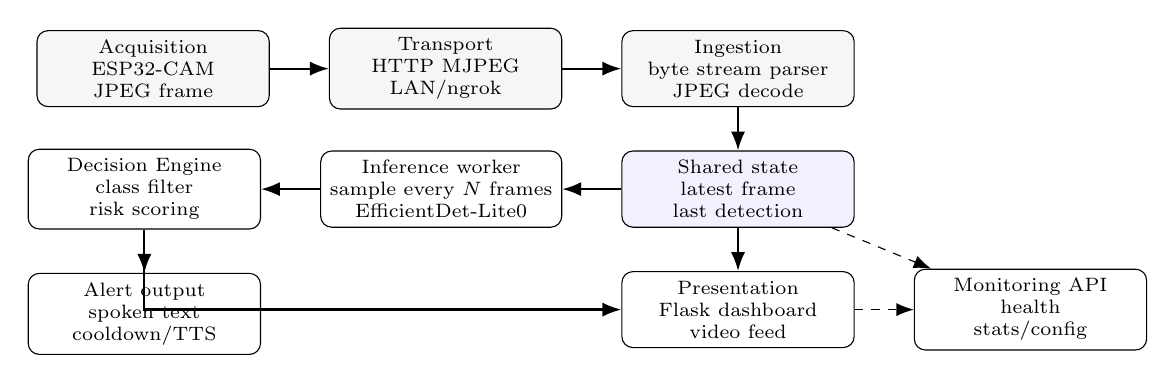
\begin{tikzpicture}[
    font=\scriptsize,
    node distance=0.55cm and 0.75cm,
    layer/.style={draw, rounded corners, align=center, minimum width=2.95cm, minimum height=0.92cm, fill=gray!7},
    service/.style={draw, rounded corners, align=center, minimum width=2.95cm, minimum height=0.92cm},
    state/.style={draw, rounded corners, align=center, minimum width=2.95cm, minimum height=0.82cm, fill=blue!5},
    arrow/.style={-{Latex[length=2.4mm]}, thick},
    control/.style={-{Latex[length=2.2mm]}, dashed}
  ]
    \node[layer] (cam) {Acquisition\\ESP32-CAM\\JPEG frame};
    \node[layer, right=of cam] (transport) {Transport\\HTTP MJPEG\\LAN/ngrok};
    \node[layer, right=of transport] (ingest) {Ingestion\\byte stream parser\\JPEG decode};
    \node[state, below=of ingest] (buffer) {Shared state\\latest frame\\last detection};
    \node[service, left=of buffer] (infer) {Inference worker\\sample every $N$ frames\\EfficientDet-Lite0};
    \node[service, left=of infer] (decision) {Decision Engine\\class filter\\risk scoring};
    \node[service, below=of decision] (alert) {Alert output\\spoken text\\cooldown/TTS};
    \node[service, below=of buffer] (dashboard) {Presentation\\Flask dashboard\\video feed};
    \node[service, right=of dashboard] (api) {Monitoring API\\health\\stats/config};

    \draw[arrow] (cam) -- (transport);
    \draw[arrow] (transport) -- (ingest);
    \draw[arrow] (ingest) -- (buffer);
    \draw[arrow] (buffer) -- (infer);
    \draw[arrow] (infer) -- (decision);
    \draw[arrow] (decision) -- (alert);
    \draw[arrow] (buffer) -- (dashboard);
    \draw[arrow] (decision) |- (dashboard);
    \draw[control] (buffer) -- (api);
    \draw[control] (dashboard) -- (api);
  \end{tikzpicture}
  \caption{Kiến trúc xử lý biên và các mặt phẳng dữ liệu/giám sát}
  \label{fig:architecture}
\end{figure}

\begin{table}[H]
  \centering
  \caption{Trách nhiệm của các khối trong kiến trúc}
  \label{tab:architecture-blocks}
  \small
  \begin{tabularx}{\textwidth}{L{3.1cm}Y}
    \toprule
    \textbf{Khối} & \textbf{Trách nhiệm thiết kế} \\
    \midrule
    Acquisition & Cấu hình sensor OV2640, lấy frame JPEG, duy trì Wi-Fi và phát endpoint \texttt{/stream}. \\
    Transport & Chuyển luồng MJPEG qua LAN; khi demo khác mạng có thể bọc bằng ngrok mà không thay đổi DADN server. \\
    Ingestion & Đọc byte stream, tách từng JPEG bằng marker SOI/EOI, decode sang frame BGR và cập nhật frame mới nhất. \\
    Inference worker & Không suy luận mọi frame; chỉ chạy mỗi $N$ frame để giảm tải CPU và giữ dashboard phản hồi được. \\
    Decision Engine & Lọc lớp vật thể liên quan, tính mức gần--xa tương đối, vùng trái--giữa--phải và chọn cảnh báo ưu tiên. \\
    Presentation/API & Render video đã overlay, hiển thị alert, cung cấp \texttt{/health}, \texttt{/api/stats} và \texttt{/api/config}. \\
    \bottomrule
  \end{tabularx}
\end{table}

\subsection{Luồng xử lý dữ liệu}
Luồng dữ liệu được tổ chức theo kiểu producer--consumer để tránh việc giao diện web bị phụ thuộc trực tiếp vào tốc độ suy luận của mô hình. Thread capture đóng vai trò producer: nó giữ kết nối tới ESP32-CAM, đọc byte stream, tách JPEG frame và cập nhật frame mới nhất vào vùng trạng thái dùng chung. Detector chỉ được gọi theo chu kỳ \texttt{INFERENCE\_EVERY\_N\_FRAMES}; giữa hai lần suy luận, dashboard vẫn có thể hiển thị frame mới và dùng lại kết quả detection gần nhất.

Quy trình data plane gồm các bước chính:
\begin{enumerate}
  \item ESP32-CAM chụp frame ở định dạng JPEG và phát dưới dạng multipart MJPEG tại \texttt{/stream}.
  \item DADN server mở kết nối HTTP tới stream URL, đọc dữ liệu theo chunk và tìm cặp marker JPEG \texttt{0xFFD8}/\texttt{0xFFD9}.
  \item Mỗi JPEG hoàn chỉnh được decode bằng OpenCV thành frame BGR. Frame mới nhất được ghi vào buffer có khóa để route web không đọc trạng thái dở dang.
  \item Cứ mỗi $N$ frame, server đưa frame vào MediaPipe Object Detector. Cách lấy mẫu này giảm tải tính toán nhưng vẫn giữ được nhịp cập nhật hình ảnh.
  \item Danh sách detection được chuẩn hóa thành \texttt{DetectionItem} rồi chuyển vào Decision Engine để tạo \texttt{ScoredObstacle}.
  \item Kết quả cảnh báo gần nhất được lưu trong shared state. Dashboard dùng trạng thái này để vẽ bounding box, thông điệp cảnh báo và thống kê FPS/inference.
  \item Nếu stream mất kết nối hoặc không đọc được chunk mới, capture loop ghi log lỗi, chờ ngắn hạn rồi thử kết nối lại thay vì làm sập Flask server.
\end{enumerate}

Luồng control/monitoring chạy song song với data plane. Endpoint \texttt{/health} dùng để xác nhận server còn sống và stream vẫn đang cập nhật; \texttt{/api/stats} phục vụ đo FPS, số frame, số lần suy luận và cảnh báo gần nhất; \texttt{/api/config} giúp ghi nhận cấu hình khi nghiệm thu. Nhờ đó, nhóm có thể phân biệt lỗi do camera, mạng, model hay dashboard thay vì chỉ nhìn một cửa sổ video bị đứng.

\section{Thiết kế Decision Engine}

\subsection{Vai trò}
Nếu đọc trực tiếp mọi nhãn mà mô hình phát hiện được, hệ thống dễ tạo ra quá nhiều thông báo và gây nhiễu cho người dùng. Decision Engine giải quyết vấn đề này bằng cách trả lời bốn câu hỏi: vật thể nào liên quan đến an toàn di chuyển, vật thể đó ở gần hay xa tương đối, nó nằm ở hướng nào trong khung hình, và vật thể nào cần được cảnh báo trước.

\subsection{Lọc lớp vật thể}
Hệ thống chỉ giữ lại các lớp có trọng số trong \texttt{CLASS\_WEIGHTS}. Các lớp này được chia thành nhóm ưu tiên theo mức ảnh hưởng đến di chuyển.

\begin{table}[H]
  \centering
  \caption{Nhóm vật thể ưu tiên cảnh báo}
  \label{tab:class-priority}
  \begin{tabularx}{\textwidth}{L{3.4cm}Y}
    \toprule
    \textbf{Nhóm} & \textbf{Ví dụ lớp vật thể} \\
    \midrule
    Ưu tiên cao & person, bicycle, motorcycle, car, bus, truck \\
    Ưu tiên trung bình & chair, bench, suitcase, potted plant, backpack \\
    Bỏ qua giai đoạn đầu & bottle, cup, remote, tv và các vật nhỏ ít ảnh hưởng đến lối đi \\
    \bottomrule
  \end{tabularx}
\end{table}

\subsection{Ước lượng mức gần--xa tương đối}
Do hệ thống dùng một camera RGB monocular, khoảng cách tuyệt đối không được đo trực tiếp. Phiên bản hiện tại dùng diện tích bounding box trên toàn frame làm tín hiệu gần--xa:
\[
AreaRatio = \frac{w \times h}{W \times H}
\]
trong đó $w, h$ là kích thước bounding box, còn $W, H$ là kích thước frame. Nếu đáy bounding box nằm ở vùng thấp của ảnh, hệ thống tăng nhẹ tỷ lệ này vì vật thể có khả năng nằm gần hướng di chuyển hơn. Ngưỡng mặc định trong \texttt{config.py} là \texttt{NEAR\_AREA\_RATIO = 0.18} và \texttt{MEDIUM\_AREA\_RATIO = 0.06}.

Cách làm này phù hợp với demo ban đầu vì đơn giản và chạy nhanh, nhưng nó chưa phải ước lượng khoảng cách hình học. Vật thể thật sự lớn có thể bị xem là gần hơn vật thể nhỏ dù hai vật ở cùng khoảng cách. Vì vậy, ở phần hướng phát triển, nhóm cần bổ sung tracking ngắn hạn hoặc mô hình depth/TTC để tăng độ tin cậy.

\subsection{Xác định hướng trái--giữa--phải}
Tâm bounding box theo trục ngang được chuẩn hóa theo chiều rộng frame. Nếu tâm nằm dưới 0.33, vật thể được xem là ở bên trái; nếu trên 0.67, vật thể ở bên phải; phần còn lại là vùng giữa. Vùng giữa được ưu tiên hơn vì thường trùng với hướng di chuyển chính của người dùng.

\subsection{Tính điểm ưu tiên}
Mỗi detection hợp lệ được chuyển thành một \texttt{ScoredObstacle}. Điểm ưu tiên được tính bằng tích của trọng số lớp, trọng số khoảng cách, trọng số vùng trung tâm, trọng số hướng và confidence:
\[
\begin{aligned}
Priority ={}& ClassWeight \times DistanceWeight \times CenterWeight \\
            & \times DirectionWeight \times Confidence
\end{aligned}
\]
Vật thể có \texttt{Priority} cao nhất được chọn làm cảnh báo chính tại thời điểm hiện tại. Cách chấm điểm dạng nhân giúp các vật thể nguy hiểm hơn, ví dụ người hoặc xe nằm gần vùng trung tâm, nổi bật hơn các vật thể ở rìa hoặc có confidence thấp.

\subsection{Sinh câu cảnh báo và chống lặp âm thanh}
Decision Engine sinh câu cảnh báo tiếng Việt theo mức gần--xa và hướng, ví dụ ``Cẩn thận, có người ở giữa, rất gần''. Module \texttt{VoiceAlertManager} dùng \texttt{pyttsx3}, lưu thông điệp gần nhất và chỉ phát lại khi qua thời gian cooldown hoặc khi mức rủi ro tăng. Trong dashboard hiện tại, \texttt{spoken\_text} được hiển thị cùng frame; khi tích hợp TTS vào luồng demo, cần ưu tiên chạy bất đồng bộ để không chặn luồng camera.

\section{Triển khai phần mềm}

\subsection{Cấu trúc module}
\begin{table}[H]
  \centering
  \caption{Vai trò các module chính trong repository}
  \label{tab:module-role}
  \small
  \begin{tabularx}{\textwidth}{L{3.6cm}Y}
    \toprule
    \textbf{Module} & \textbf{Vai trò} \\
    \midrule
    \filepath{ESP32_CAM_Project/src/main.cpp} & Firmware ESP32-CAM: khởi tạo camera, Wi-Fi, web server và MJPEG stream. \\
    \filepath{DADN/stream_server.py} & Server demo chính: đọc MJPEG stream, chạy inference nền, vẽ overlay và xuất dashboard Flask. \\
    \filepath{DADN/run_stream_server.py} & Launcher cho stream server, nhận camera URL từ tham số, biến môi trường hoặc file runtime. \\
    \filepath{DADN/detector.py} & Wrapper MediaPipe Object Detector, chuẩn hóa detection thành dataclass. \\
    \filepath{DADN/decision_engine.py} & Lọc vật thể, ước lượng gần--xa, xác định hướng, tính priority và sinh câu cảnh báo. \\
    \filepath{DADN/tts_engine.py} & Quản lý Text-to-Speech bằng \texttt{pyttsx3}, cooldown và phát lại khi mức rủi ro tăng. \\
    \filepath{DADN/api_server.py} & API nhận ảnh qua POST \texttt{/api/detect}, phù hợp nếu client gửi từng JPEG. \\
    \filepath{DADN/expose_dashboard_ngrok.py} & Chạy hoặc tái sử dụng dashboard DADN rồi expose port 5000 qua ngrok. \\
    \filepath{ESP32_CAM_Project/auto_camera_ngrok.py} & Tự dò ESP32-CAM trong LAN, mở ngrok và ghi public stream URL. \\
    \bottomrule
  \end{tabularx}
\end{table}

\subsection{Cấu hình quan trọng}
Các tham số quan trọng được gom vào \texttt{config.py}, gồm đường dẫn model, kích thước frame, chu kỳ suy luận, ngưỡng confidence, số detection tối đa, ngưỡng gần--xa, vùng trung tâm, cooldown giọng nói và nhãn tiếng Việt. Việc gom cấu hình giúp nhóm dễ tinh chỉnh khi chuyển từ laptop sang Raspberry Pi hoặc khi đổi camera.

\subsection{Dashboard và API}
Dashboard Flask cung cấp các endpoint chính:
\begin{itemize}
  \item \texttt{/}: giao diện web hiển thị stream đã overlay.
  \item \texttt{/video\_feed}: luồng MJPEG đã vẽ detection và alert.
  \item \texttt{/health}: trạng thái server, FPS, số frame và số lần suy luận.
  \item \texttt{/api/stats}: thống kê inference, cảnh báo gần nhất và cấu hình runtime.
  \item \texttt{/api/config}: cấu hình server hiện tại.
\end{itemize}

\subsection{Quy trình vận hành ESP32-CAM}
Firmware ESP32-CAM giữ Wi-Fi ở dạng placeholder để tránh lộ credential trong Git. Khi demo, người vận hành cập nhật SSID/password cục bộ, flash firmware bằng PlatformIO, mở Serial Monitor để lấy IP. URL stream sau đó được truyền cho DADN server theo dạng:
\begin{center}
  \footnotesize\ttfamily http://<ESP32\_IP>:8081/stream
\end{center}

\section{Kịch bản demo và vận hành}

\subsection{Cùng mạng LAN}
\begin{enumerate}
  \item Flash firmware ESP32-CAM và đọc Serial Monitor để lấy stream URL.
  \item Chạy DADN server với tham số \texttt{--camera-url} trỏ đến stream URL của ESP32-CAM.
  \item Mở dashboard tại \texttt{http://localhost:5000}.
  \item Kiểm tra \texttt{/health} và \texttt{/api/stats} trong quá trình demo.
\end{enumerate}

\subsection{Khác mạng hoặc demo public}
\begin{enumerate}
  \item Trên máy nhìn thấy ESP32-CAM, chạy script ngrok phía ESP32 để tạo public stream URL.
  \item Trên Raspberry Pi hoặc máy chạy model, chạy \texttt{run\_stream\_server.py} với public stream URL.
  \item Nếu cần public dashboard, chạy \texttt{expose\_dashboard\_ngrok.py} để expose port 5000.
\end{enumerate}

\section{Kiểm thử và đánh giá}

\subsection{Mục tiêu kiểm thử}
Kiểm thử nhằm xác nhận hệ thống không chỉ nhận diện vật thể, mà còn chọn đúng vật thể cần cảnh báo, xác định đúng hướng, phản ứng hợp lý với mức gần--xa tương đối và phục hồi được khi stream gián đoạn.

\begin{table}[H]
  \centering
  \caption{Kịch bản kiểm thử đề xuất}
  \label{tab:test-scenarios}
  \small
  \begin{tabularx}{\textwidth}{L{1.0cm}Y Y Y}
    \toprule
    \textbf{STT} & \textbf{Tình huống} & \textbf{Kết quả mong đợi} & \textbf{Tiêu chí đánh giá} \\
    \midrule
    1 & Một người đứng giữa lối đi ở khoảng cách gần & Cảnh báo người ở giữa hoặc phía trước & Nhận diện đúng lớp person, priority cao \\
    2 & Xe máy nằm ở mép phải khung hình & Cảnh báo xe máy bên phải nếu đủ gần & Xác định đúng vùng phải, không ưu tiên vật nhỏ khác \\
    3 & Ghế ở xa trong hành lang & Cảnh báo mức thấp hơn hoặc bỏ qua nếu không nằm trên hướng chính & Spatial fallback và vùng trung tâm hợp lý \\
    4 & Nhiều vật thể cùng lúc: người ở giữa, xe đạp ở rìa trái & Ưu tiên người ở giữa & Thuật toán chọn vật thể ưu tiên đúng \\
    5 & Stream ESP32-CAM mất kết nối & Server retry sau 2 giây và không crash & Khả năng phục hồi kết nối \\
    6 & Dashboard public qua ngrok & \texttt{/health}, \texttt{/video\_feed}, \texttt{/api/stats} truy cập được & Demo remote chạy được \\
    \bottomrule
  \end{tabularx}
\end{table}

\subsection{Chỉ số cần đo thực nghiệm}
Nhóm chưa nên ghi số liệu định lượng nếu chưa đo trực tiếp trên thiết bị demo. Các chỉ số cần cập nhật khi nghiệm thu gồm:
\begin{table}[H]
  \centering
  \caption{Bảng chỉ số thực nghiệm cần cập nhật sau khi chạy demo}
  \label{tab:metrics}
  \begin{tabularx}{\textwidth}{L{4.0cm}Y L{3.0cm}}
    \toprule
    \textbf{Chỉ số} & \textbf{Cách đo} & \textbf{Giá trị hiện tại} \\
    \midrule
    FPS trung bình & Ghi nhận FPS hiển thị hoặc \texttt{current\_fps} trong \texttt{/api/stats} trong 60 giây & Cần đo \\
    Độ trễ suy luận & Thời gian từ lúc nhận frame đến khi có danh sách detection & Cần đo \\
    Độ trễ end-to-end & Thời gian từ lúc vật cản xuất hiện đến khi dashboard/TTS hiển thị cảnh báo & Cần đo \\
    Tỷ lệ cảnh báo đúng vật thể ưu tiên & Số tình huống chọn đúng vật nguy hiểm nhất trên tổng số tình huống test & Cần đo \\
    Độ ổn định stream & Số lần reconnect trong 5 phút với LAN và ngrok & Cần đo \\
    \bottomrule
  \end{tabularx}
\end{table}

\section{Đánh giá hạn chế và rủi ro}

\subsection{Hạn chế hiện tại}
Hệ thống chưa đo được khoảng cách tuyệt đối theo mét vì chỉ dùng một camera RGB. Heuristic area ratio có thể sai khi vật thể có kích thước thật khác nhau hoặc bị crop. Decision Engine hiện chưa tracking cùng một vật qua nhiều frame, nên cảnh báo có thể dao động khi detection thay đổi. Nếu dùng ESP32-CAM qua Wi-Fi hoặc ngrok, độ trễ mạng có thể ảnh hưởng đến thời điểm cảnh báo.

Ngoài ra, \texttt{tts\_engine.py} đã tồn tại nhưng chưa phải luồng chính trong dashboard stream. Trước demo chính thức, nhóm cần xác định rõ cảnh báo giọng nói sẽ phát từ server, từ trình duyệt hay từ thiết bị ngoài.

\subsection{Rủi ro khi triển khai thực tế}
Các rủi ro quan trọng gồm cảnh báo sai lớp vật thể, bỏ sót vật cản thấp không có trong tập lớp COCO, lặp cảnh báo gây mất tập trung, và trễ tổng thể quá lớn khi người dùng di chuyển nhanh. Vì vậy, hệ thống cần được xem là công cụ hỗ trợ thử nghiệm, chưa đủ điều kiện sử dụng như thiết bị an toàn độc lập.

\section{Hướng phát triển}

Các hướng mở rộng phù hợp gồm:
\begin{itemize}
  \item Bổ sung tracking ngắn hạn để giảm nhấp nháy alert giữa các frame.
  \item Nâng cấp từ heuristic area ratio sang TTC proxy hoặc monocular depth có hiệu chỉnh.
  \item Tích hợp \texttt{tts\_engine.py} vào \texttt{stream\_server.py} theo hướng bất đồng bộ để không chặn luồng camera.
  \item Thêm trang cấu hình dashboard để nhập stream URL, inference interval và threshold mà không sửa code.
  \item Tinh chỉnh hoặc huấn luyện mô hình với dữ liệu thực tế tại Việt Nam, đặc biệt là xe máy, vỉa hè và vật cản thấp.
  \item Đo và tối ưu end-to-end latency trên Raspberry Pi thay vì chỉ kiểm tra trên laptop.
\end{itemize}

\section{Kết luận}

Đề tài đã xác định được hướng triển khai khả thi cho hệ thống cảnh báo vật cản bằng giọng nói cho người khiếm thị. Repository hiện tại đã có các thành phần chính cho demo end-to-end: ESP32-CAM phát stream, DADN server nhận frame, EfficientDet-Lite0 chạy suy luận, Decision Engine chọn cảnh báo và dashboard Flask hiển thị trạng thái. Cách tiếp cận này phù hợp với mục tiêu của đồ án đa ngành vì kết hợp phần cứng camera, mô hình AI nhẹ, xử lý phần mềm, giao diện giám sát và tương tác âm thanh.

Trong giai đoạn tiếp theo, trọng tâm cần chuyển từ hoàn thiện pipeline sang đo thực nghiệm trên thiết bị thật. Các chỉ số như FPS, độ trễ suy luận, độ trễ phát cảnh báo, độ ổn định stream và tỷ lệ cảnh báo đúng vật thể ưu tiên sẽ quyết định mức độ khả dụng của hệ thống trong môi trường thực tế.

\bibliographystyle{plainnat}
\bibliography{refs/report}

\end{document}
